\chapter{Preliminary Work}
\label{chap:preliminary-work}
\vspace{-10mm}
\section{Software architecture}
\label{sec:architecture}
\begin{figure}[H]
    \centering
    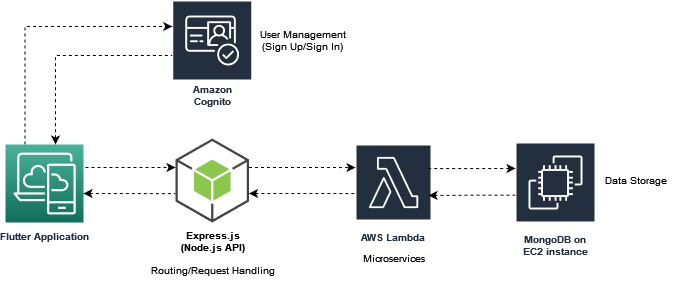
\includegraphics[width=\textwidth]{graphics/project-architecture.png}
    \caption{A high-level system architecture outlining basic interactions.}
    \label{fig:architecture-diagram}
\end{figure}
\vspace{-5mm}
Using an Express API inside AWS Lambda is beneficial because
AWS Lambda is an event-driven serverless platform. Instead of paying for cloud servers, you pay for compute power
that is proportional to the complexity of events taking place. For example,
we can process data on command instead of constantly having processes taking place.
This can cause ``cold starts'' where there is some time wasted if the system hasn't been accessed
in a while, but the time spent is negligible for our project and the cost-benefit analysis would show
that this is a rationale decision. Using Amazon Cognito also removes much of the development
time needed to create simple user management. This doesn't require much skill and so making use of 
Amazon Cognito is saving us time to use where knowledge and focus is needed.
\pagebreak

\section{User interface design}
\label{sec:UI-design}
\vspace{-3mm}
We have created some preliminary designs (\cref{fig:prototype}) in the form of a functional prototype.
Main screens have been created and the overall aesthetic is displayed.
It's highly likely that the colour palette is different to meet the brand
we decide to create behind the application.\\
The functional prototype can be found here: \href{https://www.figma.com/proto/aANVZK2JZcBTPZCzaFYvbm/Final-Year-Project-Prototype?scaling=scale-down&page-id=0%3A1&starting-point-node-id=0%3A3&node-id=0%3A3}{Project Prototype Link}.
\vspace{-2mm}
\begin{figure}[H]
    \centering
    \begin{minipage}{0.5\textwidth}
        \begin{subfigure}{\textwidth}
            \centering
            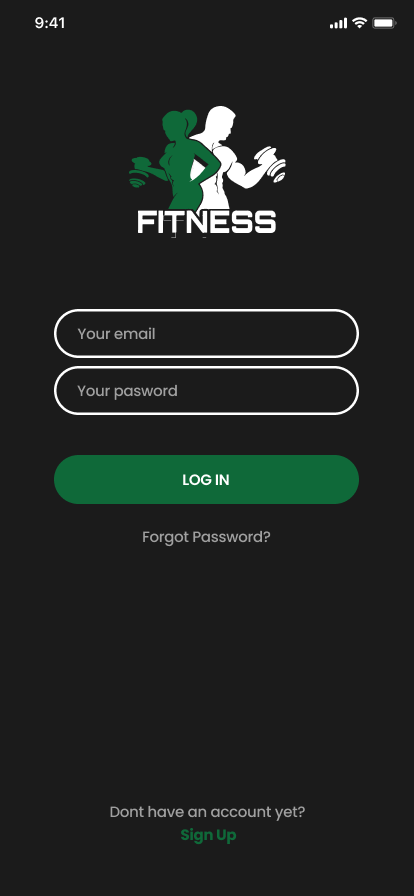
\includegraphics[width=0.45\textwidth]{graphics/prototype/login-page.png}
            \caption{Login screen}
            \label{fig:prototype-login}
        \end{subfigure}
    \end{minipage}%
    \begin{minipage}{0.5\textwidth}
        \begin{subfigure}{\textwidth}
            \centering
            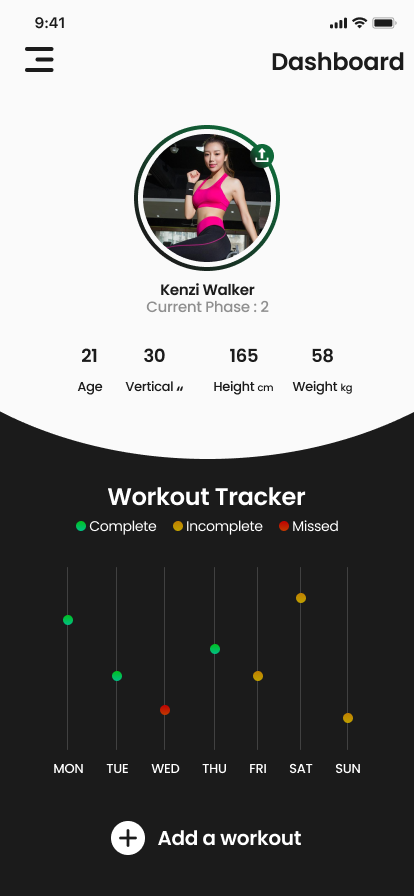
\includegraphics[width=0.45\textwidth]{graphics/prototype/dashboard.png}
            \caption{Main dashboard}
            \label{fig:prototype-dashboard}
        \end{subfigure}
    \end{minipage}\\*[3mm]
    \centering
    \begin{minipage}{0.5\textwidth}
        \begin{subfigure}{\textwidth}
            \centering
            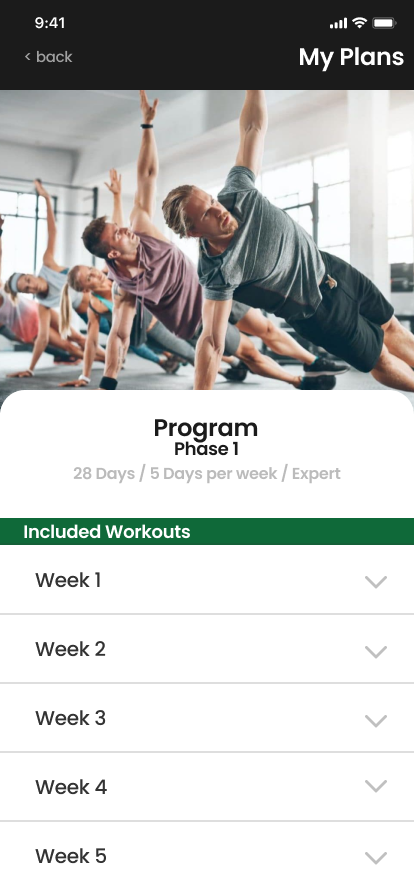
\includegraphics[width=0.45\textwidth]{graphics/prototype/workout-plan.png}
            \caption{Workout screen}
            \label{fig:prototype-workouts}
        \end{subfigure}
    \end{minipage}%
    \begin{minipage}{0.5\textwidth}
        \begin{subfigure}{\textwidth}
            \centering
            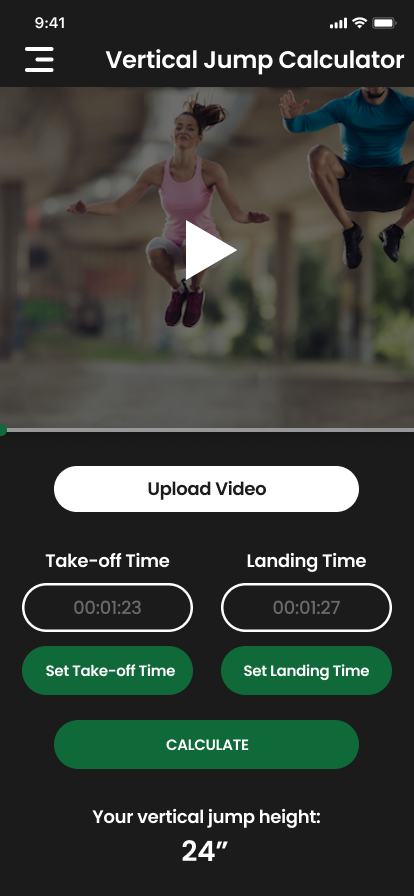
\includegraphics[width=0.45\textwidth]{graphics/prototype/jump-calc.png}
            \caption{Jump calculator screen}
            \label{fig:prototype-jump-calc}
        \end{subfigure}
    \end{minipage}%
    \caption{A selection of prototype screens.}
    \label{fig:prototype}
\end{figure}